%!TEX TS-program = xelatex
%!TEX root = ../../maxwell2018thesis.tex

\begin{tikzpicture}[remember picture, overlay]
      \node[anchor=north west] at (-2.88,3.475){%
        \scalebox{0.66}{\pgfimage{figures/ch0-acks_header.pdf}}};
\end{tikzpicture}

\begin{preamble}[The PhD Journey]
\setcounter{footnote}{0}
\phantomsection
\addcontentsline{toc}{part}{The PhD Journey}

A good friend of mine (and a fellow PhD student) once said to me that when the time came to write his PhD thesis, he would avoid an acknowledgements section where \emph{everyone and their dog} would be thanked for helping him reach his target of attaining a PhD. I, on the other hand, hold a very different opinion on this matter. There are a lot of people, who have in one way or another, helped me reach where I am today. Whether these people actively guided me in my studies, or were individuals who I was fortunate to become acquainted with over the past five years, they all \emph{``cajoled''}\footnote{Professor Ian Ruthven used this term in his PhD thesis~\citep{ruthven2001phd} as a means of describing the individuals who were there for him, behind the scenes, \emph{``cajoling''} him towards the finishing line.} me in one way or another towards the finishing line.

I firmly believe that everybody who I have the pleasure of meeting and working with over the past five years should be acknowledged -- whether they feel they contributed in any meaningful way. If you are one of these people and are left wondering, believe me: \emph{you did make a difference.} While acknowledgements may not merit enough gratitude to those who have helped me along the way, I still wish to thank all of you. \textbf{\emph{To show my sincere appreciation, I want to dedicate this work to each and every one of them}} -- regardless of whether they have a dog or not.

Hindsight tells me that doing a PhD is much like embarking on a \emph{very long,} solo journey. Unless you have experienced it yourself, you won't appreciate how tough (and lonely) it can be at times -- especially when things don't go according to plan. Three years in, I found myself sitting in my lab all alone on a Friday night, wondering why my experiments weren't producing the results I had expected and hoped for.\footnote{It was a stupid mistake, of course. From memory, I think I forgot to increment a counter in a loop. But it took an entire evening to figure that out. \emph{Of course it did!}} It can at times all seem so incredibly pointless, and you find yourself questioning what you're doing with your life. I experienced these lows more times than I care to admit. It can be tortuous. \emph{Impostor syndrome} is something every PhD student feels, and I was no exception.

However, I got to the finishing line. Doing a PhD isn't just about learning your field of study and making an original contribution to it; no, it's much more than that. It also involves learning about yourself. It's \emph{character building.} It involves steely grit and determination to get through the difficult times. Even when everything comes crashing down around you, \emph{you will get through it.} My PhD taught me this more than anything, and for that I am incredibly thankful. I'm definitely a different person for having done it\footnote{This is something most people will agree with. My friend James gave a nod to this in the acknowledgements of his excellent PhD thesis, too~\citep{mcminn2018phd}.} -- a much better one (I think so, anyway!), equipped with a good skillset to enter the world and make a positive contribution. Even though every PhD comes complete with negative moments, I took positives from all of them. From this, I could enjoy the good times even more. And believe me, there were \emph{heaps} of good times during the past five years.

One of the many great things about my experience as a PhD student was the office I was given to work in. It's in the \emph{Sir Alwyn Williams Building (SAWB),} room 221. Being a contemporary building, there are lots of windows -- and you get a really nice view of the grass next to Lilybank Gardens, looking down to \emph{Brel}, and, yeah, the \emph{Boyd Orr Building,} too. However, in moments of reflection, I always found myself staring vacantly out the window at people walking past outside, going about their lives. Everyone's experiences -- from all walks of life -- are different, making for a virtually limitless number of stories to listen to, and to learn from. I have always found this truth about life to be absolutely fascinating.

So, on that basis, I want to spend the next few pages writing about \emph{my PhD journey,} acknowledging everyone who made a positive impact along the way. I think that investing the additional time in writing this short passage is a good reflective experience, and also goes a little to say thanks for the amazing things these people have done for me.

I hope you enjoy reading it as much as I enjoyed writing it.

%\acksep

\blueboxheader{Day One \textemdash~and Looking Back}
Day one was October 1\textsuperscript{st}, 2013. I remember this day well. In particular, I have vivid memories of sitting down at my new desk in the morning and thinking something along the lines of \emph{``what have I just let myself in for?!''}. The very idea that I was now a PhD student in itself felt really daunting because from reading research papers in my MSci year, I was humbled by how much knowledge there was out there -- and I had to get myself to a level to contribute to that knowledge. After being assigned my first task by my supervisor, Leif, I set to work -- but it did seem very overwhelming.

However, I chipped away at it. As one task was completed, the next one fell into place -- and I found I could do that, too (with some guidance, of course!). I started to produce things, got a paper accepted after six months, and presented it at a conference (as I'll talk about shortly). But as I worked away, I started to find another area of research\footnote{User modelling and simulation -- the scope of this thesis.} to be much more interesting. The work presented in the thesis you are reading is actually pretty different from what I thought about doing back on day one. It just goes to show how when you think you have something laid out before you, it's by no means certain that it'll happen.

\blueboxheader{Life in Glasgow}
One constant that was present throughout my time as a PhD student at Glasgow was the people. There were always individuals I could rely on for support, advice, or a simple chat. We'd often find ourselves down at Brel when the sunshine was out (which did happen \emph{sometimes}). These are the people that I'd like to acknowledge first -- and what better than to start with those who I shared an office with over the past five years?

\blueboxheader{SAWB221}
To Stuart Mackie, {\arabicfont الصافوري ابراهيم امين فاطمه} (Fatma Elsafoury), my \emph{tocayo} Jorge David Gonz\'{a}lez Paule and {\asianfont 王烯} (Xi Wang) -- thank you for your companionship throughout the years in \emph{SAWB221.} The camaraderie and support we gave one another did not go unnoticed, and I am grateful for that. Fatma, thank you for the support and interesting philosophical discussions that we had. There are also two other individuals with whom I also shared \emph{SAWB221} with -- and also a home (for four years!). To Hora\c{t}iu Bota, thank you for the friendship that we had over the years throughout our time as PhD students. To {\thaifont \Large จรณะ มโนธรรมรักษา} (Jarana Manotumruksa), thank you for your friendship throughout. It's been an absolute pleasure, and it didn't feel like being in an office -- you all made it a happy place.

I'd also like to say thank you to my friends Colin McLellan and Andrew (James) McMinn. All three of us started at the \emph{University of Glasgow} back in September 2008 as undergraduates in Computing Science. Colin was in my very first \emph{CS1Q} undergraduate lab! By early 2019, all three of us had passed our PhD defences at the same institution, although the routes we took to get to that point were slightly different. \emph{We got through it together!} To Colin in particular, thank you for the support and friendship -- especially when we were both writing up at the end. Having the same supervisor kept us in close contact with one another -- but I don't think either of us has a bad word to say about Leif!

\blueboxheader{Team IR}
With all of us working on some aspect of IR, there's also more people within the wider IR group that I would like to acknowledge. My appreciation goes out to everyone who resided next door in \emph{SAWB220} over the years, including {\arabicfont  الخوالدة سليمان رامي} (Rami Alkhawaldeh), {\arabicfont الدبعي عبدالرقيب شوقي} (Shawki Al-Dubaee), {\arabicfont العشبان ابراهيم نجود} (Nujud Aloshban), Phil McParlane, Jes\'{u}s Alberto Rodriguez P\'{e}rez (and his brother, F\'{e}lix Rodr\'{i}guez P\'{e}rez), Stewart Whiting, {\asianfont 辛鑫} (Xin Xin) and {\asianfont 发杰原} (Fajie Yuan). To Stewart in particular, thank you for your support throughout your time as a PhD student -- your guidance was greatly appreciated and valued when I started out. You made things seem a little less daunting.

I'd also like to acknowledge those in the rest of the IR group at Glasgow. In particular, I would like to acknowledge Dr Jeff Dalton, Professor Joemon Jose, Dr Craig Macdonald, Dr Richard McCreadie, Graham Mcdonald, {\asianfont 方安杰} (Anjie Fang) and {\asianfont 苏亭} (Ting Su) for their friendship and support throughout the years. Professor Iadh Ounis in particular was a source of great support. Together with Leif and Craig, Iadh taught me many of the basics of IR in my MSci year, for which I am very grateful. Iadh was also one of the examiners for my final PhD defence -- and I'll talk about that experience later.

I'd also like to pay particular thanks to {\farsifont مشفقى ياشار} (Yashar Moshfeghi) for his friendship and support throughout my time at Glasgow. When you and Guido Zuccon were both PhD students at Glasgow, you were my tutors for the undergraduate \emph{Java Programming 2} course -- and you both helped to reinforce many of the programming constructs that I use today! Yashar, your expert knowledge and advice on how to run crowdsourced studies was also appreciated. You played an important role in helping me to get the user studies that I define and report on in this thesis up and running. Thank you.

\blueboxheader{Glasgow Computing Science}
Of course, I didn't just exclusively interact and socialise with people who studied IR. One of the great things about the \emph{School of Computing Science} at the University of Glasgow is its size and the huge range of different disciplines that are studied. I have made friends with many people along the way, and also learnt things from different research areas, too. It's always interesting to see what other people are working on.

I made some close friends. To G\"{o}zel Shakeri, you are the best. I cannot thank you enough for your friendship, support and encouragement that you've given me throughout my time as a PhD student. The support and words of advice through the difficult times -- especially when my world came crashing down in mid-2018 -- will not be forgotten. Even if I was able to even begin offering you the advice and comfort that you did for me, I will have been a good friend to you, too. And to Frances Cooper, thanks for your friendship and company, especially when you had a brief stay in \emph{SAWB221} during my final writeup phase!

\renewcommand{\figurename}{Picture}
\begin{wrapfigure}[9]{r}{0.45\textwidth}
    \begin{center}
    \vspace*{-9mm}
    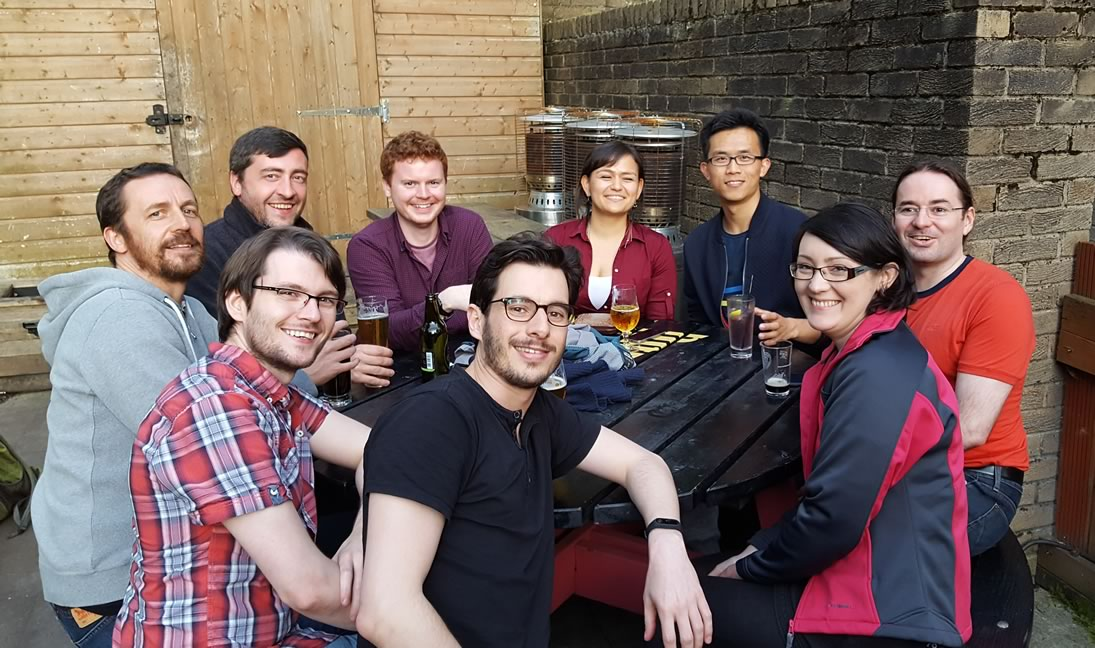
\includegraphics[width=1\textwidth]{figures/ch0-brel.jpg}
    \end{center}
    \vspace*{-6mm}
    \caption{The good old days, back in August 2016. Sl\'{a}inte, everyone!}
    \label{fig:acks_friends}
\end{wrapfigure}
\renewcommand{\figurename}{Figure}

In addition to G\"{o}zel and Frances, there are heaps of other people at Glasgow that I want to acknowledge. To name a few... Blair Archibald, Dr Ornela Dardha, Наталья Чечина (Dr Natalia Chechina), Marco Cook, Richard Cziv\'{a}, Euan Freeman, Simon Jouet, Φωτεινή Κατσαρού (Foteini Katsarou), William Kavanagh, Antoine Loriette, Ciaran McCreesh, Stephen McQuistin, Magnus Morton, Алекс Панчева (Alex Pancheva), Craig Reilly, Stefan Raue, Dr Giorgio Roffo, Charlie Rutherford, Kyle Simpson, Robbie Simpson, Dr Michel Steuwer, Lovisa Sundin, Patrizia Di Campli San Vito, Tom Wallis, Dr David White and Михаил Янев (Mihail Yanev) -- you all over the years provided a friendly face and support. My appreciation goes out to every single one of you. Even if we simply had a chat and/or a drink, your company meant (and still means!) a lot.

I would also like to thank Professor Roderick Murray-Smith. Thank you for your support when Leif left Glasgow in mid-2016 to the \emph{University of Strathclyde.} Your insightful advice and feedback gave me an alternative perspective from which I viewed my work. I was able to incorporate some of your points into the final product, making it a stronger thesis.

And to those friends from outside the School, I want to acknowledge your support and continued friendship. In particular, I'd like to acknowledge Julie Briand, Gary Christie, Ad\'{e}la Holubov\'{a}, Nick Swan and Shaun Rew. Julie, thanks for your company throughout the process -- we both achieved our goals and got our PhDs! \emph{``Choose your future. Choose life.''} I'd also like to mention Sean McKeown -- thank you Sean for your friendship throughout the whole experience. I value your advice and feedback, and I hope I have been able to repay that over the years. You have done \emph{Edinburgh Napier} proud.

\blueboxheader{Tutoring, Exam Collection and More}
I always said to my friends that when my PhD work was getting tough, I could find some solace in teaching. Throughout my time as a student in the School of Computing Science, I've been incredibly fortunate to take on such important roles -- and from those roles, meet and work with some fantastic people. Back when I was a fourth year undergraduate, Professor Quintin Cutts introduced me to the world of teaching. From that moment, I never looked back. Tutoring and demonstrating were some of the best things I did at Glasgow. Sitting down and helping someone understand a solution to a problem that they have been facing in their work was such an enjoyable experience.

I tutored labs for a total of \emph{nine years} -- and loved every minute of doing so. While I tutored basics such as \emph{CS1P} and \emph{JP2} (Python and Java programming), my main focus was undoubtedly \emph{web development.} As I'll talk about later, I wrote a book with Leif called \emph{Tango with Django} to make learning the \emph{Django} web application framework a more straightforward experience. I'd like to thank Professor David Manlove and Dr Gerardo Arag\'{o}n-Camarasa for providing me with the opportunity to continue working on web development with them in my capacity as a tutor. I thoroughly enjoyed working with you both. And to my friend and fellow PhD student Laura Voinea, thank you for your company during the \emph{WAD2} and \emph{ITECH} labs over the years. Working with you was an absolute pleasure.

Of course, there's also the administrative team within the School that kept things flowing smoothly. These were the individuals who supported me when I needed it, too -- and I want to acknowledge them here. To Lydia Marshall, Helen McNee and Αναστασία Φλιάτουρα (Anastasia Fliatoura), thank you for making everything as straightforward as it could have been, at least from an administrative point of view! In particular, I want to thank Anastasia for her help in sorting out the thesis submission dates for me at the end of the PhD.

I also want to acknowledge Teresa Bonner, Helen Border and Gail Reat in the teaching office. You all trusted me to do the job that I did when it came to tutoring, and for that, I am very grateful. One of the other jobs you gave me during my time as a PhD student was to run around the campus during exam season and collect the student's scripts. Although to many this sounds like a nightmare, I actually really enjoyed it. Once again, it provided a nice break from my studies, and I learnt how to sort \textasciitilde 200 exam scripts by matriculation number in the quickest possible time. \emph{Where else would I have got that experience?} Thanks also to Magnus and Laura -- as well as Paul Harvey -- for your companionship when we spent those days in April-May 2015, 2016 and 2017 running around collecting all the student's scripts!

Of course, all of these extra commitments I took onboard were for the benefit of the students who have studied at the School over the years. As one of their tutors/demonstrators, I've had the good fortune to get to know some wonderful people over the years. Even if I guided them through their studies for a few weeks of their lives, I hope that I left an impact.

In particular, I want to acknowledge Екатерина Александрова (Ekaterina Aleksandrova), Lisa Brooks, {\asianfont 陳文勝} (Winston Chen), Άγγελος Κωνσταντινίδης (Angelos Constantinides), David Creigh, Tom Decke, Ивелина Дойнова (Ivelina Doynova), Leisha Hussein, Lisa Laux, Elena Lucchetti, Rebekka Orth, Gabriele Rossi, Vincent Schlatt and Tevhide Turkmen for keeping in touch and your friendship throughout our time here at Glasgow. It has been a pleasure. Sorry that you were inflicted with the pain of having to \emph{Tango with Django} -- but I know that in the end, you all tangoed really well!

\blueboxbold{Broadening my Horizons}
I had many fantastic times in the School of Computing Science. But one of the perks of being a PhD student is the ability to travel. I had the good fortune to travel for conferences, internships and summer schools. I was originally uneasy at the idea of travelling solo, but after travelling to my first conference, this fear totally disappeared. Travelling became one of my favourite things to do, and I relished the opportunity to visit a new city, country, or continent -- and of course to meet new people.

The different flags at the start of this section show the countries I visited throughout my studies. Of particular fondness to me are the memories of my first conference in Amsterdam, The Netherlands \emph{(ECIR 2014)} -- and the conference where I did my first presentation, at \emph{IIiX 2014} in Regensburg, Germany. It went alright, and I have now given numerous talks about my work all over the world. Although I always feel nervous about doing them beforehand, they always turn out alright. Maybe I'll learn to calm my nerves one day.

However, individuals that I met helped me put my mind at ease, and made me realise that what I was doing was worthy. At the first \emph{CHIIR} conference in North Carolina, USA, I participated in the Doctoral Consortium. Dr Jaap Kamps for being my mentor. Thank you Jaap for offering me insightful advice for shaping up my work. I'd also like to acknowledge Dr Mark Smucker for the discussion and words of encouragement he gave at the conference.

\renewcommand{\figurename}{Picture}
\begin{wrapfigure}[11]{r}{0.45\textwidth}
    \begin{center}
    \vspace*{-9mm}
    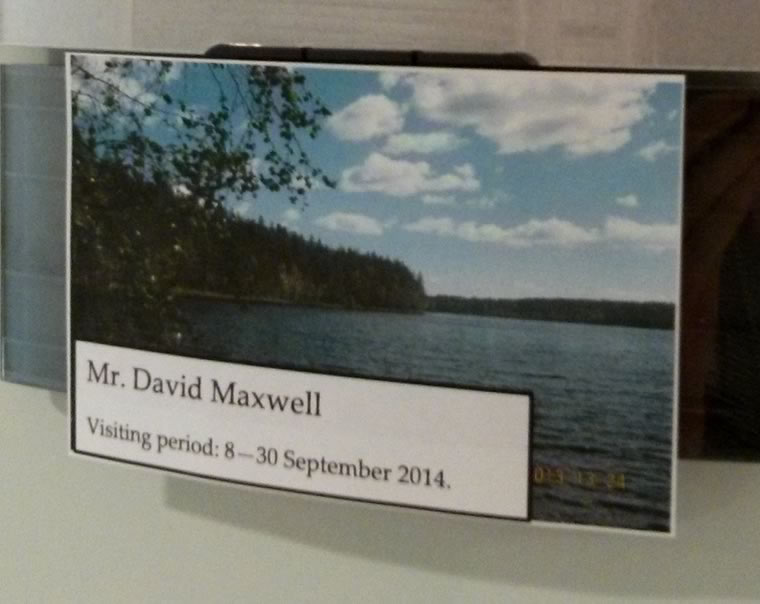
\includegraphics[width=1\textwidth]{figures/ch0-tampere.jpg}
    \end{center}
    \vspace*{-6mm}
    \caption{My name on the door at \emph{Tampereen yliopisto!}}
    \label{fig:acks_finland}
\end{wrapfigure}
\renewcommand{\figurename}{Figure}

Support also came from Finland in the shape of a \emph{Short-Term Scientific Mission (STSM)}.\footnote{This was funded by the \emph{MUMIA COST Action}, grant \#\texttt{ECOST-STSM-IC1002-080914-049840}.} I was fortunate enough to spend several weeks at the \emph{University of Tampere} back in September 2014 with Professor Kalero J\"{a}rvelin, Dr Feza Baskaya, Dr Jaana Kek\"{a}l\"{a}inen, Dr Heikki Keskustalo and Teemu P\"{a}\"{a}kk\"{o}nen. I am very grateful for the guidance and friendship I received during my stay in Tampere. It was a successful trip, too -- the simulation framework \simiir~that was used in this thesis makes use of some of the querying strategies that were devised at Tampere, and our work stemmed several interesting collaborations that led to publications at conferences such as \emph{CIKM 2015.}

A further collaboration saw me pay a short visit in November 2015 to the \emph{University of Duisburg-Essen} in Germany. Here, I was fortunate enough to work with Professor Norbert Fuhr and my friends Trần Tuấn Vũ and Ιωάννης Καρατάσης (Ioannis Karatassis) on modelling the search process using Markov models. It was an interesting and rewarding time, with a further publication presented at \emph{ICTIR 2017.} I am grateful to all involved for the kindness shown during my stay in Germany. Thank you.

I also interned during the summer of 2017 at the \emph{Alan Turing Institute (ATI)} in London. During this time, I learnt more about mathematics, and contributed to other areas of science. I'm grateful that I was able to apply my computing science knowledge on different problems and would like to thank Professor Terry Lyons and Dr Hao Ni for their guidance throughout the project I undertook with my teammates, Alex Cioba and Rados\l{}aw Kowalski. Acknowledgements also go to the other wonderful people at the ATI who were there with me, including James Bell, William Kayat, Tim King, Emily Neilson, Bernardo P\'{e}rez Orozco, Dr Jeremy Reizenstein and {\asianfont 石海忱} (Haichen Shi) -- as well as my friend Dr David White and Faustyna Krawiec for making life outside the ATI during that summer so enjoyable.

\renewcommand{\figurename}{Picture}
\begin{wrapfigure}[9]{r}{0.45\textwidth}
    \begin{center}
    \vspace*{-9mm}
    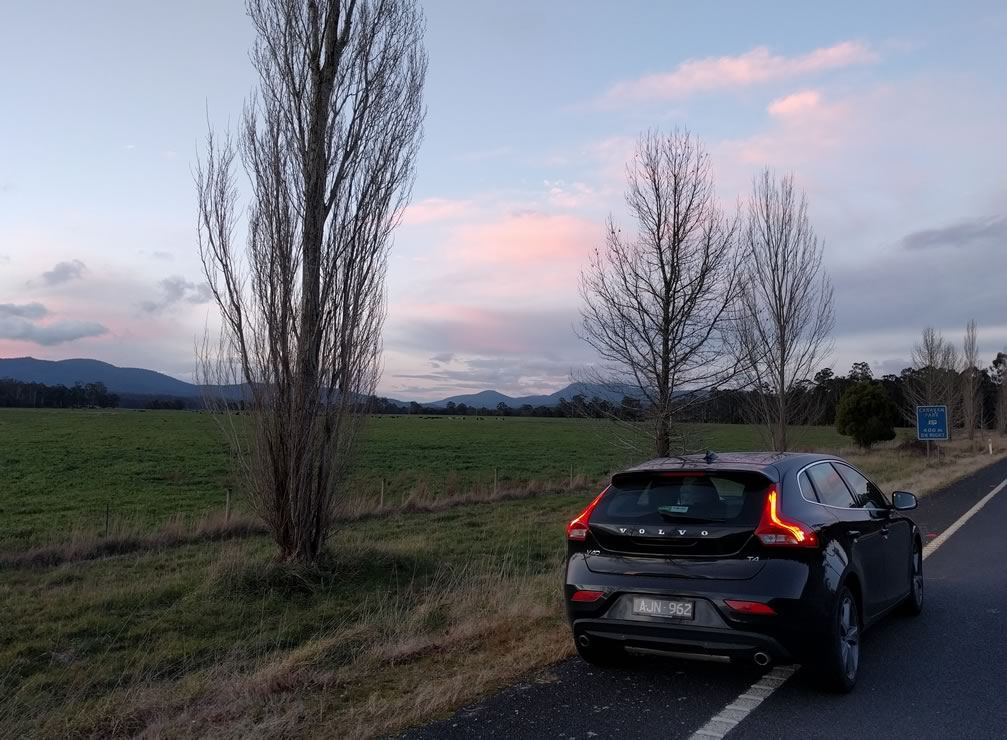
\includegraphics[width=1\textwidth]{figures/ch0-aus.jpg}
    \end{center}
    \vspace*{-6mm}
    \caption{Melbourne $\rightarrow$ Canberra.}
    \label{fig:acks_australia}
\end{wrapfigure}
\renewcommand{\figurename}{Figure}

However, one of the places that I travelled to that stands out the most in my mind was Australia. In the last quarter of 2016, I had a wonderful time in Canberra working at \emph{Microsoft} with the company of Dr Peter Bailey, Professor Dave Hawking and Dr Paul Thomas (along with Dr Nick Craswell, who was based over in Bellevue, Washington). During my time in Canberra, I learnt so much -- not only about how things at Microsoft work, and how to collaborate, but also about myself. The experience was superb, and I wouldn't have had it any other way. To Peter, Dave and Paul -- thank you for the kindness and support you showed me during my time there. It was an absolute pleasure working with you all, and I hope that I was suitably able to demonstrate my skills.

Before heading to Canberra however, I visited Melbourne. I'd like to thank my friends Johanne Trippas and Πηνελόπη Αναλυτή (Penny Analytis) for their kindness and hospitality for the first few days of my Australian adventure. I hope I can repay that one day. Driving from Melbourne up to Canberra, although \emph{very} long, was one of my highlights. And once I was at my destination, I didn't look back. I remember the nervousness about approaching a random table of young people in a Canberran bar in an attempt to make friends. I am happy to report that I did it -- and in the process gained some fantastic friends! Through my friends in Canberra, I learnt how to bachata -- although I think I could definitely have spent some more time practising. I would like to thank James Dart, Gabrielle McGill and Alan Wu for their friendship and support. In particular, I'd like to thank James and Gabrielle for their continued support, and showing me around Sydney. Gabrielle, your country is absolutely amazing -- and I'd love to pay a return visit soon.

Indeed, making friends and connections with others was a common theme throughout my travels. It was a brilliant time, and I look back on every place I went to with fond memories. There are so many people that I met during my time as a PhD student, but several people stand out in my mind. These people include {\burmesefont ညီညီထွန်း} (Nyi-Nyi Htun), {\asianfont 김은정} (Eunjeong Kim), {\asianfont 三井マット} (Matthew Mitsui), {\armenianfont Հասմիկ Օսիպյան} (Hasmik Osipyan), Maya Sappelli, Maria Han Veiga and {\asianfont 유주완} (Juwan Yoo). Maria, I hope we get to meet again soon! And in particular, I'd like to thank {\farsifont دهقانی مصطفا} (Mostafa Deghani) and {\farsifont آب‌نار سمیرا} (Samira Abnar) for their amazing company and hospitality in Amsterdam when my travel plans fell apart.

\blueboxbold{The Highs and Lows}
It goes without saying that the places I mentioned are associated with good times. However, doing a PhD is not a linear process, and I think it's also important to acknowledge that \emph{things didn't always go to plan, either.} As I said back at the start, it's a character building process. I took a positive from every negative experience, and I hope that I'm a stronger individual for having been through the tough times.

Experiments went wrong. Conference deadlines were always a stressful experience. Despite my best planning, I would always find myself staying up late the night before the deadline. One of the lowest points came in early 2017 when after weeks of hard graft, I realised that all of the experimental results for a \emph{CIKM 2017} paper on simulation were totally bogus. It was heartbreaking -- but Leif was understanding, and I was able to pick myself back up, fix the problems I identified, and submit the revised work to \emph{ECIR 2018} instead. This kind of thing is something I am surprised I don't hear more of amongst PhD students, because everyone makes mistakes. And from each mistake, you learn something new.

I'd be lying if I said things were straightforward elsewhere in my life, too. The writeup phase is already a difficult and stressful (but somewhat enjoyable) process -- and when things went wrong elsewhere in mid-2018, it was a tough pill to swallow. It happens. But I am grateful for my friends (who I have acknowledged) for helping me through that bad period. I got there! And I am grateful to them for helping me get to this point.

\blueboxbold{The Final Defence}
\emph{Getting there} led to the \emph{final PhD defence.} I submitted my thesis a few months prior, and it felt like 1,000 tonnes had been lifted from my shoulders. The pressure came back, however, before the final defence. I was super apprehensive about it -- \emph{what if I was asked a question I had no idea about?}

However, it was alright! I heard several of my friends who had been through the process in the months leading up to my defence, saying that the process was actually \emph{enjoyable.} I would agree completely. I knew my stuff -- having just written a thesis on it -- and the questions I was asked were fair and reasonable. It was confidence-inspiring, and when questioned by my examiners, I felt like an \emph{equal to them.} It was an enlightening experience, and I am all the better for having completed it successfully.

To that end, I'd like to say thank you to my two examiners, Professor Iadh Ounis and Dr Suzan Verberne. I am humbled by the warm and encouraging feedback you both gave me on the work I have done, and I hope you enjoyed reading the thesis -- and asking me questions on it, too! My thanks also to the convenor of my defence, Dr Michele Sevegnani.

\blueboxbold{Closer to Home}
Of course, three of the individuals who I owe the most two are my parents and brother. To my mother, Denise, and my father, William: thank you from the bottom of my heart for the love and support that helped me get to 2019, where I can call myself \emph{Doctor Dave.} You've both told me that I have done you proud, and I hope that I can continue to do so as I try to figure out my own way through life. The sacrifices that you both made for myself and Alastair have not gone unnoticed, and I am (and I know Alastair is!) eternally grateful for the opportunities that you have both provided us.

To my brother Alastair, thanks for everything you've done for me -- especially over the past five years. You've been a strong voice of reason to counter my sometimes clouded judgement, and you've helped steer me through murky waters. Your excellent proofreading abilities are also acknowledged, and I have to thank you for taking the time to read this thesis as I finished chapter after chapter. Keep doing what you're doing. I love you all.

I'd also like to pay tribute to someone who also strongly encouraged me to get into computing -- and along with my parents, helped kickstart the idea of attending university in the first place. To Ian Phillips, my computing teacher at \emph{Mearns Castle High School} -- thank you. You saw me through Standard Grade and Advanced Higher Computing, and you were another individual who was conducive in helping me get to where I am today.

\blueboxbold{My Supervisor}
However, there's one more individual I deliberately saved until the end. Without his guidance and support, I am certain I wouldn't be where I am today. Dr Leif Azzopardi was my PhD supervisor, and he also saw me through my fourth and fifth year undergraduate projects. He also taught me many of the IR and programming concepts that I put to good use in this work, and taught me new ways to look at the world.

From the first time I met him as one of my lecturers in 2011, Leif has offered me nothing but absolute support and encouragement. He took the time out of his day to discuss the problems I was facing and warmly welcomed me to his family. He offered me support when I needed it, and never lost his trust in me -- even when I lost some trust in myself. And with that trust in me came so many opportunities, perhaps chief of which was co-authoring \emph{Tango with Django} with him, a book that has been used by thousands and thousands of people around the world. He provided me with the ability to travel and meet so many of the fantastic individuals that I have acknowledged in this passage.

Leif, you treated me as an equal throughout, and I look up to you. I would echo Colin in saying that you were both a supervisor and a trusted friend throughout the entire process, and hope that you will continue to be. \textbf{\emph{From the bottom of my heart, thank you for everything you have done for me.}} I hope that we can continue to work together in the future.

\vspace*{4mm}
\acksep

I will admit that writing this passage took far longer (and \emph{is} longer) than I envisaged. However, as I said at the beginning, I think it's important to acknowledge all of those who played a part in the journey of my PhD -- from my supervisor, to all of the friends that I made.

A total of 1,962 days passed from commencing my PhD to successfully defending it in front of Iadh and Suzan. In that time, I've learnt so much -- not only about my field of study, but about how the world works. When I left Canberra for the last time in 2016, my friend Gabrielle said to me that even though I really wanted to go back, I'd find that while the buildings would look similar, the place wouldn't feel the same to me. \emph{People move on.} They move on to different places and to do different things. And although this is true, the memories and experiences that I have gained from this five year journey will stay with me for the rest of my days. There's been plenty of ups and downs, yes. It's been a hell of a ride. But I wouldn't change a single thing.

And you know what?

\textbf{\emph{This is only the beginning!}}~\raisebox{-.2\height}{
\includegraphics[height=5mm]{figures/ch0-smile.pdf}}

\fundingfootnote{I would also like to acknowledge my funder, the \emph{EPSRC} (under grant number \texttt{1367507}). The scholarship I was provided with allowed me to complete my work without any financial headaches.}

\end{preamble}